\documentclass[openany]{article}
\usepackage{lmodern}
\usepackage{amssymb,amsmath}
\usepackage{ifxetex,ifluatex}
\usepackage{fixltx2e} % provides \textsubscript
\ifnum 0\ifxetex 1\fi\ifluatex 1\fi=0 % if pdftex
  \usepackage[T1]{fontenc}
  \usepackage[utf8]{inputenc}
\else % if luatex or xelatex
  \ifxetex
    \usepackage{mathspec}
  \else
    \usepackage{fontspec}
  \fi
  \defaultfontfeatures{Ligatures=TeX,Scale=MatchLowercase}
\fi
% use upquote if available, for straight quotes in verbatim environments
\IfFileExists{upquote.sty}{\usepackage{upquote}}{}
% use microtype if available
\IfFileExists{microtype.sty}{%
\usepackage{microtype}
\UseMicrotypeSet[protrusion]{basicmath} % disable protrusion for tt fonts
}{}
\usepackage{hyperref}
\hypersetup{unicode=true,
            pdftitle={Systems Pathology: Hemolymphatic},
            pdfauthor={Russell Fraser},
            pdfborder={0 0 0},
            breaklinks=true}
\urlstyle{same}  % don't use monospace font for urls
\usepackage{natbib}
\bibliographystyle{apalike}
\usepackage{longtable,booktabs}
\usepackage{graphicx,grffile}
\makeatletter
\def\maxwidth{\ifdim\Gin@nat@width>\linewidth\linewidth\else\Gin@nat@width\fi}
\def\maxheight{\ifdim\Gin@nat@height>\textheight\textheight\else\Gin@nat@height\fi}
\makeatother
% Scale images if necessary, so that they will not overflow the page
% margins by default, and it is still possible to overwrite the defaults
% using explicit options in \includegraphics[width, height, ...]{}
\setkeys{Gin}{width=\maxwidth,height=\maxheight,keepaspectratio}
\IfFileExists{parskip.sty}{%
\usepackage{parskip}
}{% else
\setlength{\parindent}{0pt}
\setlength{\parskip}{6pt plus 2pt minus 1pt}
}
\setlength{\emergencystretch}{3em}  % prevent overfull lines
\providecommand{\tightlist}{%
  \setlength{\itemsep}{0pt}\setlength{\parskip}{0pt}}
\setcounter{secnumdepth}{5}
% Redefines (sub)paragraphs to behave more like sections
\ifx\paragraph\undefined\else
\let\oldparagraph\paragraph
\renewcommand{\paragraph}[1]{\oldparagraph{#1}\mbox{}}
\fi
\ifx\subparagraph\undefined\else
\let\oldsubparagraph\subparagraph
\renewcommand{\subparagraph}[1]{\oldsubparagraph{#1}\mbox{}}
\fi

%%% Use protect on footnotes to avoid problems with footnotes in titles
\let\rmarkdownfootnote\footnote%
\def\footnote{\protect\rmarkdownfootnote}

%%% Change title format to be more compact
\usepackage{titling}

% Create subtitle command for use in maketitle
\providecommand{\subtitle}[1]{
  \posttitle{
    \begin{center}\large#1\end{center}
    }
}

\setlength{\droptitle}{-2em}

  \title{Systems Pathology: Hemolymphatic}
    \pretitle{\vspace{\droptitle}\centering\huge}
  \posttitle{\par}
    \author{Russell Fraser}
    \preauthor{\centering\large\emph}
  \postauthor{\par}
      \predate{\centering\large\emph}
  \postdate{\par}
    \date{2020-09-28}

\usepackage{booktabs}
\usepackage{booktabs}
\usepackage{longtable}
\usepackage{array}
\usepackage{multirow}
\usepackage{wrapfig}
\usepackage{float}
\usepackage{colortbl}
\usepackage{pdflscape}
\usepackage{tabu}
\usepackage{threeparttable}
\usepackage{threeparttablex}
\usepackage[normalem]{ulem}
\usepackage{makecell}
\usepackage{xcolor}

\begin{document}
\maketitle

{
\setcounter{tocdepth}{2}
\tableofcontents
}
\section*{About}\label{about}
\addcontentsline{toc}{section}{About}

These notes are a fairly comprehensive collection of information to
complement the lectures and labs delivered in Systems Pathology, on the
topic of the hemolymphatic system. Although all of the information is
useful, certain areas will have been emphasized in lecture. Let the
areas focussed on in lectures and lab guide your studying. There are a
few rare conditions that are not discussed in these notes, and you are
encouraged to read through the relevant chapters in the textbooks
recommended below.

The notes are available online at
\url{http://russfraser.ca/hemolymphatic/}, as a PDF on Moodle, and as an
Epub (E-book format, suitable for a tablet or e-reader). Please feel
free to provide feedback, whether on content, style, or typos!

\subsubsection*{Contact me}\label{contact-me}
\addcontentsline{toc}{subsubsection}{Contact me}

Please don't hesitate to get in touch if you have any questions.

\begin{itemize}
\tightlist
\item
  Phone: 902-620-5183
\item
  E-mail: \href{mailto:rufraser@upei.ca}{\nolinkurl{rufraser@upei.ca}}
\item
  Office: 414N, Dept. of Pathology and Microbiology
\end{itemize}

\subsection*{Reference material}\label{reference-material}
\addcontentsline{toc}{subsection}{Reference material}

\begin{itemize}
\tightlist
\item
  Zachary, J. F., \& McGavin, M. D. (2016). Pathologic Basis of
  Veterinary Disease Expert Consult. Elsevier Health Sciences.
\item
  Maxie, G. (2015). Jubb, Kennedy \& Palmer's Pathology of Domestic
  Animals-E-Book (Vol. 3). Elsevier Health Sciences.
\end{itemize}

\subsection*{Acknowledgements}\label{acknowledgements}
\addcontentsline{toc}{subsection}{Acknowledgements}

These lecture notes were prepared in R \citep{R-base} using the bookdown
\citep{xie2015}, knitr \citep{R-knitr}, and Rmarkdown
\citep{R-rmarkdown} packages. Source material was taken from
\citet{zachary2016pathologic} and \citet{maxie2015jubb}. I gratefully
acknoweldge the prior course notes from Dr.~Shannon Martinson. Images
are attributed throughout the text; unattributed images are either mine
or were found in the public domain.

\section{Introduction}\label{intro}

The hemolymphatic system is composed of the hematopoietic system, cells
within the circulation, and the lymphoid system. The hematopoietic
system is largely restricted to the bone marrow, while the cells of the
circulation are found not only in the blood, but often migrate into
tissues. The lymphoid system is widely distributed and is part of
several organs, including the lymph nodes, spleen, and various
distributed ``associated lymphoid tissues'' (ALTs), such as the mucosal
associated lymphoid tissue (MALT), bronchiolar associated lymphoid
tissues (BALT), etc., etc. Regardless of the location of the lymphoid
tissue, it's normal immunological reaction is the same.

The separation of topics in this section is a bit artificial, and could
easily be organized differently. The presentation here is the way in
which it makes most sense to me, but you may find the organization in
the reference textbook more to your liking. The information is the same.

\section{Bone marrow}\label{bone-marrow}

\subsection{Introduction}\label{introduction}

Bone marrow is found within the spongy portions of bones. It is the site
of production of the cellular elements of blood, known as hematopoiesis,
which can be broadly divided into \textbf{myeloid and lymphoid}
components. The lymphoid lineage produces lymphocytes, while the myeloid
lineage produces everything else (Fig \ref{fig:bm}). The massive number
of cells produced by the bone marrow all originate from a common stem
cell, which has the potential to differentiate into any type of cell
type found in the blood. The first division commits a stem cell either
to the \emph{lymphoid} or \emph{myeloid} lineage. Under the influence of
growth factors and cytokines, they gradually differentiate as they
divide, eventually becoming a fully differentiated, functional
leukocyte, erythrocyte, or thrombocyte. Early stages of differentiation
are morphologically indistinguishable, and the cells at this stage are
often refered to as ``blast'' cells, short for the various names of
immature cells (e.g.~monoblast, myeloblast, rubriblast, etc.). The bone
marrow is composed of cells of a variety of maturational stages, but
\textbf{mature, morphologically identifiable cells outnumber immature
``blast'' cells significantly.}

\begin{figure}

{\centering \includegraphics[width=1\linewidth]{images/bm} 

}

\caption{Schematic illustrating the progressive maturation of the various lineages of circulating blood cells.}\label{fig:bm}
\end{figure}

The location of hematopoiesis changes as an animal grows. \emph{In
utero}, the primary sites of hematopoiesis are the liver and spleen. In
neonatal and young animals, the marrow spaces of virtually all bones is
occupied and generating cells. In adults, hematopoietic tissue is mostly
restricted to axial bones (i.e.~skull, vertebrae, ribs, sternum, and
pelvis), as well as the proximal portion of the humerus and femur. As
the hematopoietic tissue receds during aging, it is replaced by fat.

Because the products of hematopoeisis are easily evaluated by sampling
the blood, \protect\hyperlink{biopsy-of-the-bone-marrow}{biopsy or
aspirate of the bone marrow} is relatively uncommon. Similarly, because
evaluation of the blood can reveal quite a bit about the underlying bone
marrow, \emph{many of the diseases of bone marrow are better evaluated
by clinical pathologists}.

\subsection{Adaptations of growth}\label{adaptations-of-growth}

\hypertarget{hyperplasia}{\subsubsection{Hyperplasia}\label{hyperplasia}}

Hyperplastic bone marrow is a common finding. \textbf{The bone marrow
responds to abnormally low levels of circulating cells by ramping up
production of that particular cell type.} Thus, many causes of anemia,
inflammation, or thrombocytopenia can lead to marrow hyperplasia.
Occasionally, the marrow cannot prodyuce the required cells. For
example, the production of red blood cells (RBCs) requires
iron-containing hemoglobin. In patients that are iron deficient,
producing new RBCs is not possible, and thus hyperplasia will not occur.

Grossly, the typically fatty portion of the marrow (i.e.~the diaphysis
of the long bones) changes from yellow to red. \textbf{Hyperplasia of
ANY cell line, not just the erythroid cell line, turns the marrow red}.

\subsubsection{Hypoplasia}\label{hypoplasia}

Bone marrow hypoplasia refers to the decrease in or absence of
production in one or more cell lines. Causes are numerous and varied.
Lack of signals for growth and differentiation can lead to hypoplasia.
For example, erythropoietin (EPO) stimulates differentiation and
production of RBCs from the marrow. EPO is produced by the kidney. In
cases of chronic renal disease, EPO production can decrease, leading to
a concurrent decrease in the cells of the erythroid lineage
(i.e.~erythroid hypoplasia). Lack of nutrients can lead to hypoplasia of
one or more cell lines. To continue the example from the
\protect\hyperlink{hyperplasia}{section on hyperplasia}, an absence of
iron leads to an inability of the erythroid lineage to mature, and can
result in hypoplasia.
\protect\hyperlink{degeneration-and-necrosis}{Degeneration and
necrosis}, which itself has a number of causes, can lead to bone marrow
hypoplasia.

Grossly, hypoplastic bone marrow is reflected by an increase in the pale
yellow component of the marrow and decrease in the red portion.

\subsubsection{Serous atrophy}\label{serous-atrophy}

Serous atrophy of fat refers to the transformation of the normal fat
component of the bone marrow into a gelatinous, transluscent material.
\textbf{It is common, and usually associated with malnutirtion or
cachexia}. It is a non-specific indicator that the animal is chronically
ill.

\hypertarget{degeneration-and-necrosis}{\subsection{Degeneration and
necrosis}\label{degeneration-and-necrosis}}

Degeneration and necrosis of the bone marrow, depending on the extent,
can have significant consequences for the animal. The most common
presenting sign is a cytopenia in one or more cell lines. Recall that
hematopoietic cells are metabolically and mitotically active: this
renders them susceptible to a wide variety of insults. However, so long
as the target of damage is not the hematopoietic stem cell (Fig
\ref{fig:bm}), it is likely that the bone marrow will be capable of
recovering, so long as the insult is removed.

Common causes of bone marrow damage include:

\begin{enumerate}
\def\labelenumi{\arabic{enumi}.}
\tightlist
\item
  Damage from radiation
\item
  Infectious agents

  \begin{itemize}
  \tightlist
  \item
    Feline immunodeficiency virus, feline leukemia virus, feline
    panleukopenia
  \item
    Equine infectious anemia virus
  \item
    Canine parvovirus 2
  \end{itemize}
\item
  Immune-mediated diseases
\item
  Idiopathic
\item
  Toxins and drugs

  \begin{itemize}
  \tightlist
  \item
    Certain chemotherapeutic agents
  \item
    Idiosyncratic drug reactions
  \item
    Toxic substances
  \end{itemize}
\end{enumerate}

\subsection{Neoplasia}\label{neoplasia}

Before diving into this section, some explanation is needed. What is
going to be discussed here are neoplasms that arise primarily from the
precursor cells within the bone marrow itself, namely leukemias. A
broader classification system uses the umbrella term ``hematopoietic
neoplasia'' to define neoplasms that arise from any of the formed
elements of blood. Thus, for example, a cutaneous mast cell tumour would
be considered a hematopoietic neoplasm, because it is caused by a cell
originally from the bone marrow, even though it forms a tumour in the
skin. \textbf{These types of tumours will not be discussed here, but
will be discussed in other sections}. A list of tumours \emph{not}
discussed here includes:

\begin{itemize}
\tightlist
\item
  Mast cell tumours (skin or GI)
\item
  Plasmacytomas (skin)
\item
  Cutaneous histiocytomas (skin)
\end{itemize}

\protect\hyperlink{primary-neoplasia}{Lymphoma} is a very important
disease, and is discussed in the section on lymph nodes (though it could
arguably be included here.)

Broadly, neoplasms of the marrow are separated based on their lineage of
origin. Neoplasms of lymphoid origin include lymphoid leukemias,
\protect\hyperlink{primary-neoplasia}{lymphoma}, and plasma cell
tumours. Neoplasms of the myeloid lineage include myeloid leukemias,
myelodysplastic syndrome, histiocytic tumours, and mast cell tumours.

\subsubsection{Myeloid neoplasms}\label{myeloid-neoplasms}

\hypertarget{acute-myeloid-leukemia-aml}{\paragraph{Acute myeloid
leukemia (AML)}\label{acute-myeloid-leukemia-aml}}

AML is defined as an acute cytopenia accompanied by \textgreater{} 20 \%
blast cells in either the blood or bone marrow (or both). Recall that
blast cells are immature cells that cannot be reliably identified by
cytology or histopathology (in other words, it is a precursor cell that
has not differentiated enough to have recognizable features).
Cytopathologists are best suited to evaluate the number of blast cells,
while histopathology of the bone marrow is useful to characterize the
extent of myelopthisis (replacement of normal marrow elements by other
tissues), and/or necrosis and fibrosis. In an ideal world, the type of
AML could be further categorized by looking for specific differentiating
markers on the neoplastic blast cells; in reality, the cost is still
high, and utility of doing so is debatable.

Animals with AML typically present with significant acute, non-specific
illness. Routine bloodwork often reveals cytopenia of one or more cell
line that cannot be explained. Peripheral blood may or may not contain
blast cells, in which case evaluation of the bone marrow by cytology or
histopathology needs to be pursued. The liver and/or spleen may be
diffusely enlarged in some cases. The prognosis for animals with AML is
very poor.

\paragraph{Myelodysplastic syndrome}\label{myelodysplastic-syndrome}

Myelodysplastic syndrome present primarily in cats and dogs as an acute,
non-specific illness. Bloodwork demonstrates one or more
non-regenerative cytopenias and dysplasia of cells either in the blood
or bone marrow. The bone marrow contains an increased proportion of
blast cells, between 5 - 20 \%. A variety of subclassifications exist.
Non-regenerative anemia is frequently present. \textbf{In dogs, MDS
often preceeds AML}.

\paragraph{Myeloproliferative neoplasms (chronic
leukemia)}\label{myeloproliferative-neoplasms-chronic-leukemia}

This is a very rare condition in animals, and is characterized by the
slow accumulation of very large numbers of well-differentiated cells of
the myeloid lineage. It is typically an incidental finding on routine
bloodwork in older animals. Very large numbers of erythrocytes,
thrombocytes, or various leukocytes may be noted in the blood. Other
peripheral cytopenias are rare, and the bone marrow is not necessarily
affected.

\subsubsection{Lymphoid neoplasms}\label{lymphoid-neoplasms}

\paragraph{Acute lymphoid leukemia
(ALL)}\label{acute-lymphoid-leukemia-all}

ALL is the lymphoid equivalent to
\protect\hyperlink{acute-myeloid-leukemia-aml}{AML}. It is characterized
by \textgreater{} 20 \% of lymphoid blasts in the circulation and/or
bone marrow. One or more cytopenias are usually noted on CBC, and there
may be involvement of the liver or spleen. Feline leukemia virus is a
predisposing factor in cats. In dogs, B-cell ALL is more common than
T-cell. In dogs, ALL can enlarge lymph nodes, and it can be difficult to
distinguish from a specific subtype of lymphoma.

Clinical signs are vague and non-specific, but are usually acute in
onset. Prognosis is very poor.

\paragraph{Chronic lymphoid leukemia}\label{chronic-lymphoid-leukemia}

\textbf{This is the most common type of leukemia in dogs}. Most are of
T-cell origin. This is an indolent form of leukemia, with a slow
accumulation of lymphocytes either within the bone marrow (B-cell origin
CLL) or spleen (T-cell origin CLL). Eventually the disease manifests
with a profound lymphocytosis. Prognosis is fair to good, with most
animals living 1 - 3 years after the diagnosis.

\paragraph{Multiple myeloma}\label{multiple-myeloma}

Multiple myeloma is a \textbf{malignant tumour of plasma cells}, usually
found in older animals. Dogs, and less frequently horses and cats, are
affected. Tumours usually appear within the medulla of bones with active
bone marrow, frequently the vertebrae and pelvis, leading to pain,
weakness, or paresis. The tumours are \textbf{osteolytic.} As you might
expect from a plasma cell tumour, the neoplastic cells secrete large
quantities of a clonal immunoglobulin, which can be easily detected on
routine bloodwork as a hypergammaglobulinemia. With electrophoresis, it
can be determined that it is a \textbf{monoclonal gammopathy}.
Proteinuria is also common, as the tumour produces free immunoglobulin
light chains that freely pass through the glomerulus, known as
\textbf{Bence-Jones proteins}. The diagnosis of multiple myeloma
requires identification of not just the neoplastic cells within the bone
marrow, but also monoclonal gammopathy, Bence-Jones proteinuria, or
osteolysis.

In cats, osteolysis is not common, and the tumour more often appears in
the abdominal organs or skin.

\hypertarget{biopsy-of-the-bone-marrow}{\subsection{Biopsy of the bone
marrow}\label{biopsy-of-the-bone-marrow}}

Marrow biopsy is somewhat rarely performed in daily clinical practice.
There is nothing preventing you from biopsying the marrow, but it
\emph{is} difficult. You need proper equipment and technique. The
relatively uncommon need for biopsy leads to clinician discomfort with a
procedure they rarely perform. Along those lines, many cases with
indications for bone marrow work-up end up being referred to specialty
centers, where specialists end up performing the biopsies.

Work-up of the bone marrow should \textbf{always include three
submissions: 1) bone marrow biopsy, 2) bone marrow aspirate, and 3) CBC
from the time of biopsy.} Any historical CBCs should be also made
available to the pathologists.

Biopsies are routinely taken from the humerus, femur, or ilium in small
animals. In large animals, the sternum and tuber coxae are preferred
sites. Aspirates and biopsies can be performed simultaneously. Bone
marrow aspirates are delivered to clinical pathologists, who can best
characterize and classify the aspirated cells. Core biopsies are sent to
anatomic pathologists, who can identify architectural disturbances and
the presence of abnormal marrow components, such as myelofibrosis,
neoplasia, or inflammation.

\emph{\textbf{A note on terminology:} This is an ``FYI'' part of the
notes, but may be useful to know. The terminolgy surrounding the
evaluation of bone marrow has changed in recent years. One of the
important metrics used to evaluate bone marrow is the ratio between
cells of the granulocytic and macrophage lineages vs.~those in the
erythrocytic lineage. Historically, this was referred to as the
``myeloid:erythroid'' ratio (M:E ratio). This is inaccurate, however, as
techinically both erythroid and granulocytic cells are part of the
myeloid lineage. The terminology has now shifted, such that this
evaluation is reported as the ``granulocytic:erythroid ratio''. If you
see the older, ``M:E'' term in the literature, it is referring to the
same thing as the ``G:E'' ratio. Fascinating stuff.}

\section{Spleen}\label{spleen}

\subsection{Review}\label{review}

Diseases involving the spleen are relatively common in dogs, but less so
in other species.

The spleen is a complex organ composed of two physical and functional
spaces: the red and white pulp. It serves three main functions:

\begin{enumerate}
\def\labelenumi{\arabic{enumi}.}
\tightlist
\item
  Filtering out aged or altered RBCs and blood-borne particulate matter.
\item
  Screening blood for pathogens.
\item
  Storage of blood (RBCs and platelets in particular)
\end{enumerate}

As with other organs, reviewing the normal structure and function of the
spleen will help you understand the pathogenesis of the conditions
described below. Chapter 13 of Pathologic Basis of Veterinary Disease
provides a good overview, and can be accessed from the library.

A few key points are worth mentioning here, however.

\begin{itemize}
\tightlist
\item
  The spleen is made up of red and white pulp.
\item
  The white pulp is composed of the periarteriolar lymphoid sheath
  (PALS), the germinal centers, and the marginal zone.
\item
  The red pulp is composed of the splenic cords, vascular sinuses, and
  macrophages, lymphocytes, plasma cells, and erythrocytes.
\item
  There is no lymph supply to or from the spleen.
\end{itemize}

Broadly, think of the spleen as a screening and filtering organ. The
blood is screened for pathogens and aged RBCs, and inappropriate
organisms or material are filtered out.

\subsection{Examination of the spleen}\label{examination-of-the-spleen}

When examining the spleen, take care to note the size (enlarged vs
normal vs small), the presence of nodules, any areas of discolouration,
and any changes in texture. The spleen should be serially sectioned:
cross-sectional slices approximately 1 cm thick made through the entire
spleen from head to tail.

Small spleens are generally unimportant. Splenic aplasia is extremely
rare, and unlikely to be encountered.

Large spleens (``splenomegaly'') are of greater concern. Large spleens
may be diffusely enlarged, or enlarged by single or multiple nodules. On
cut-section, they may be bloody (i.e.~ooze blood on cut section), or
`meaty' (i.e.~enlarged by something other than blood). Although there is
overlap between these phenotypes, broadly classifying spleens in this
way can help narrow down a list of differential diagnoses ((Table
\ref{tab:spleen-ddx}).

\begin{table}[!h]

\caption{\label{tab:spleen-ddx}Differential diagnoses for different types of splenomegaly (not an exhaustive list)}
\centering
\begin{tabular}{>{\raggedright\arraybackslash}p{10em}>{\raggedright\arraybackslash}p{10em}>{\raggedright\arraybackslash}p{10em}}
\toprule
Features & Nodular & Diffuse\\
\midrule
**Bloody** & [Hematoma],
                                        [hemangiosarcoma][Hemangiosarcoma],
                                        [acute splenic infarct][Necrosis and infarction],
                                        incomplete splenic contraction & [Congestion],
                                        splenic torsion,
                                        [septicemia][Sepsis],
                                        hemolytic anemia\\
**Meaty** & [Nodular hyperplasia],
                                        [various sarcomas][Non-angiomatous, non-lymphomatous sarcomas],
                                        metastatic neoplasia,
                                        [granulomas][Chronic splenitis] & Histiocytic sarcoma[Hemophagocytic histiocytic sarcoma],
                                        [leukemia/lymphoma][Lymphoma],
                                        amyloidosis\\
\bottomrule
\end{tabular}
\end{table}

\subsection{Circulatory disturbances}\label{circulatory-disturbances}

\subsubsection{Congestion}\label{congestion}

With their enormous capacity to store blood, spleens can vary
tremendously in size. Congestion leads to an enlarged spleen that oozes
blood on cut section. The most common cause of an enlarged, congested
spleen is \textbf{barbituate euthanasia}, but splenic torsion, acute
hemolytic anemia, or shock can also lead to a congested spleen.

\hypertarget{hematoma}{\subsubsection{Hematoma}\label{hematoma}}

Hematomas are common masses found in the spleen, particularly of dogs.
They can range greatly in size, from 1 - 2 cm up to very large, 20 - 30
cm masses. They are dark red, poorly demarcated from the adjacent
splenic parenchyma, and are bloody on cut section. They may be caused by
trauma, or by alteration of the circulatory system caused by other
benign growths, such as \protect\hyperlink{nodular-hyperplasia}{nodular
hyperplasia}. Rupture of theses masses can lead to hemoabdomen and
hypovolemic shock. \textbf{These masses cannot be grossly differentiated
from \protect\hyperlink{hemangiosarcoma}{hemangiosarcoma}, and thus must
be submitted for histopathology}.

\subsubsection{Necrosis and infarction}\label{necrosis-and-infarction}

\textbf{Infarctions} are common lesions found in the spleen. Due to the
nature of the vascular supply of the spleen, there is little collateral
circulation, rendering them prone to infarction. Acute venous infarcts
(Fig \ref{fig:spleen-infarct-acute}) generally appear bright red, well
demarcated, and may bulge slightly on cut section. As the infarct
matures, the necrotic tissue is removed and replaced by fibrous
connective tissue (Fig \ref{fig:spleen-infarct}), and becomes pale and
firm (in other words, the spleen develops a scar).

\begin{figure}

{\centering \includegraphics[width=1\linewidth]{images/20-18021-canine-spleen-necrosis-2} 

}

\caption{Irregularly arborizing areas of deep red are noticable along the surface of this spleen, consistent with acute necrosis.}\label{fig:spleen-infarct-acute}
\end{figure}

\begin{figure}

{\centering \includegraphics[width=1\linewidth]{images/spleen-infarct-3-black} 

}

\caption{Along the left lateral aspect of this cross-section of a spleen, there is a pale white, well demarcated area consistent with a chronic infarct}\label{fig:spleen-infarct}
\end{figure}

Although splenic infarctions are often incidental findings, they may be
key lesions in certain diseases. Infectious diseases causing vascular
damage, for example classical swine fever virus or sepsis, can lead to
infarction. Hypercoagulable states, seen with immune-mediated hemolytic
anemia or as a paraneoplastic syndrome, can result in infarction.
Endocarditis (bacterial infection of the heart valves) can result in
septic emboli or in thrombi, which can lodge in the small vessels of the
spleen and lead to infarction.

\subsection{Inflammation and
infection}\label{inflammation-and-infection}

Unlike some other tissues (for example, liver or lung), infections only
rarely settle and become chronic in the spleen, perhaps due to the large
numbers of phagocytic cells. The spleen, however, can react to
blood-borne pathogens, or to pathogens that target lymphoid tissues. A
few examples of each are discussed below.

\subsubsection{Sepsis}\label{sepsis}

Given its role in filtering the blood, it is understandable that the
spleen would react to massive blood-borne infections of sepsis. In some
instances of sepsis, the spleen is markedly enlarged by blood, soft, and
dark red.

\paragraph{Anthrax}\label{anthrax}

Anthrax is important not because it is a frequent disease (its rare),
but because it is \textbf{fatal to many animals, including humans} (it's
also \textbf{reportable}). It is caused by \emph{Bacillus anthracis}, a
gram-positive, spore-forming bacteria. Herbivores in particular are
susceptible, while reptiles and carnivorous birds are resistant.
Infection is generally acquired through the disturbance of soil
(e.g.~excavation), which exposes the spores that are \emph{highly
resistant to the environment, and can live for long periods (years) in
adverse conditions}. Cattle and sheep ingest spores, and spores enter
circulation through traumatized mucous membranes. Carnivores may become
infected by consuming the carcass of an infected herbivore, or through
direct consumption of the spores. Following ingestion, the spores
germinate and traffic to lymph nodes, causing a lymphangitis and
lymphadenitis that then progresses to septicemia. The bacteria produce 3
key toxins: \textbf{edema factor, lethal factor, and protective
antigen}. These toxins contribute to vascular damage and impaired
coagulation, along with injury and inactivation of phagocytes.
\textbf{Death is usually rapid (\textless{} 24 hours), especially in
sheep and goats.} Cattle may also die rapidly, but some probably
recover.

The classical presentation of a case of bovine anthrax is sudden death
of the animal with little to no clinical signs. The animal will often
\textbf{ooze blood from its orifices}, and will appear to have putrified
more rapidly than expected. \textbf{Marked splenomegaly is common}, and
blood fails to clots.

There are 2 reasons why you will hopefully never see the splenomegaly
associated with anthrax. 1) It is a rare (and zoonotic!) disease. 2)
\textbf{You should not necropsy an animal you suspect is affected with
anthrax}.

To elaborate on point 2: massive replication of \emph{B. anthracis} in
the host occurs prior to death. \textbf{Upon exposure to air, the
organisms sporulate, forming the highly resistant organisms that can
contaminate the environment}. Thus, instead of necropsying these animals
and getting anthrax spores all over the place, a blood smear taken prior
to necropsy can identify the organisms. Rapid body-side test kits for
\emph{B. anthracis} are also available.

\subsubsection{ASFV and CSFV}\label{asfv-and-csfv}

African swine fever (ASF) virus and classical swine fever (CSF) virus
are two \textbf{reportable diseases} of swine. They both affect a
variety of organs, and the spleen is one. Both diseases cause lymphoid
depletion. CSF often leads to hemorrhagic infarcts, while ASF causes
marked splenomegaly.

\subsubsection{Chronic splenitis}\label{chronic-splenitis}

This is relatively uncommon. Granulomas, presenting either as multifocal
pale nodules or a diffusely pale spleen, can be caused by
\emph{Mycobacterium} spp. and systemic fungal diseases such as
histoplasmosis or blastomycosis.

Splenic abscesses are similarly uncommon. \emph{Rhodococcus equi} (in
horses) is perhaps the most common agent, along with \emph{Truperella
pyogenes} (cattle).

\subsection{Hyperplasia and neoplasia}\label{hyperplasia-and-neoplasia}

Neoplastic diseases of the spleen present either as nodules or as a
diffusely enlarged, meaty (but not bloody) spleen. The former is more
common. \textbf{It is not possible to differentiate grossly between
nodular lesions on the spleen},
\protect\hyperlink{biopsying-the-spleen}{biopsy} and submitting them for
histopathology is the only way to diagnose these masses.

The most important neoplasm of the spleen is
\protect\hyperlink{hemangiosarcoma}{hemangiosarcoma}.

\hypertarget{nodular-hyperplasia}{\subsubsection{Nodular
hyperplasia}\label{nodular-hyperplasia}}

Nodular hyperplasia is a common finding in the spleens of dogs, and to
some degree bulls. Nodular hyperplasia simply refers to the
proliferation of elements of the spleen to the extent that they form a
nodule. The elements may be lymphoid in origin (lymphoid nodular
hyperplasia), may be foci of extramedullary hematopoeisis, or may have a
mixture of varying components. They are benign lesions, but can be
difficult to grossly differentiate from hemangiosarcoma. They are
usually small (up to 2 cm, but can be larger), and often have irregular
areas of palor on cut-section. They may be a predisposing factor for the
development of a \protect\hyperlink{hematoma}{splenic hematoma}.

\hypertarget{hemangiosarcoma}{\subsubsection{Hemangiosarcoma}\label{hemangiosarcoma}}

\textbf{Hemangiosarcoma is the most common malignant neoplasm of the
spleen in dogs}, and is almost invariably fatal. \textbf{There is no
cure}. The cause of the disease is uncertain, but likely multifactorial.

The gross appearance of hemangiosarcoma is variable (see Fig
\ref{fig:hemangio}). The neoplasm may appear as one or multiple nodules,
some of which may be ruptured. It is not uncommon for a portion of the
omentum to adhere to ruptured nodules. Nodules are generally diffusely
red or mottled red and white, bloody on cut section, and are poorly
demarcated from the adjacent spleen. Larger nodules are often necrotic
at their core.

\begin{figure}

{\centering 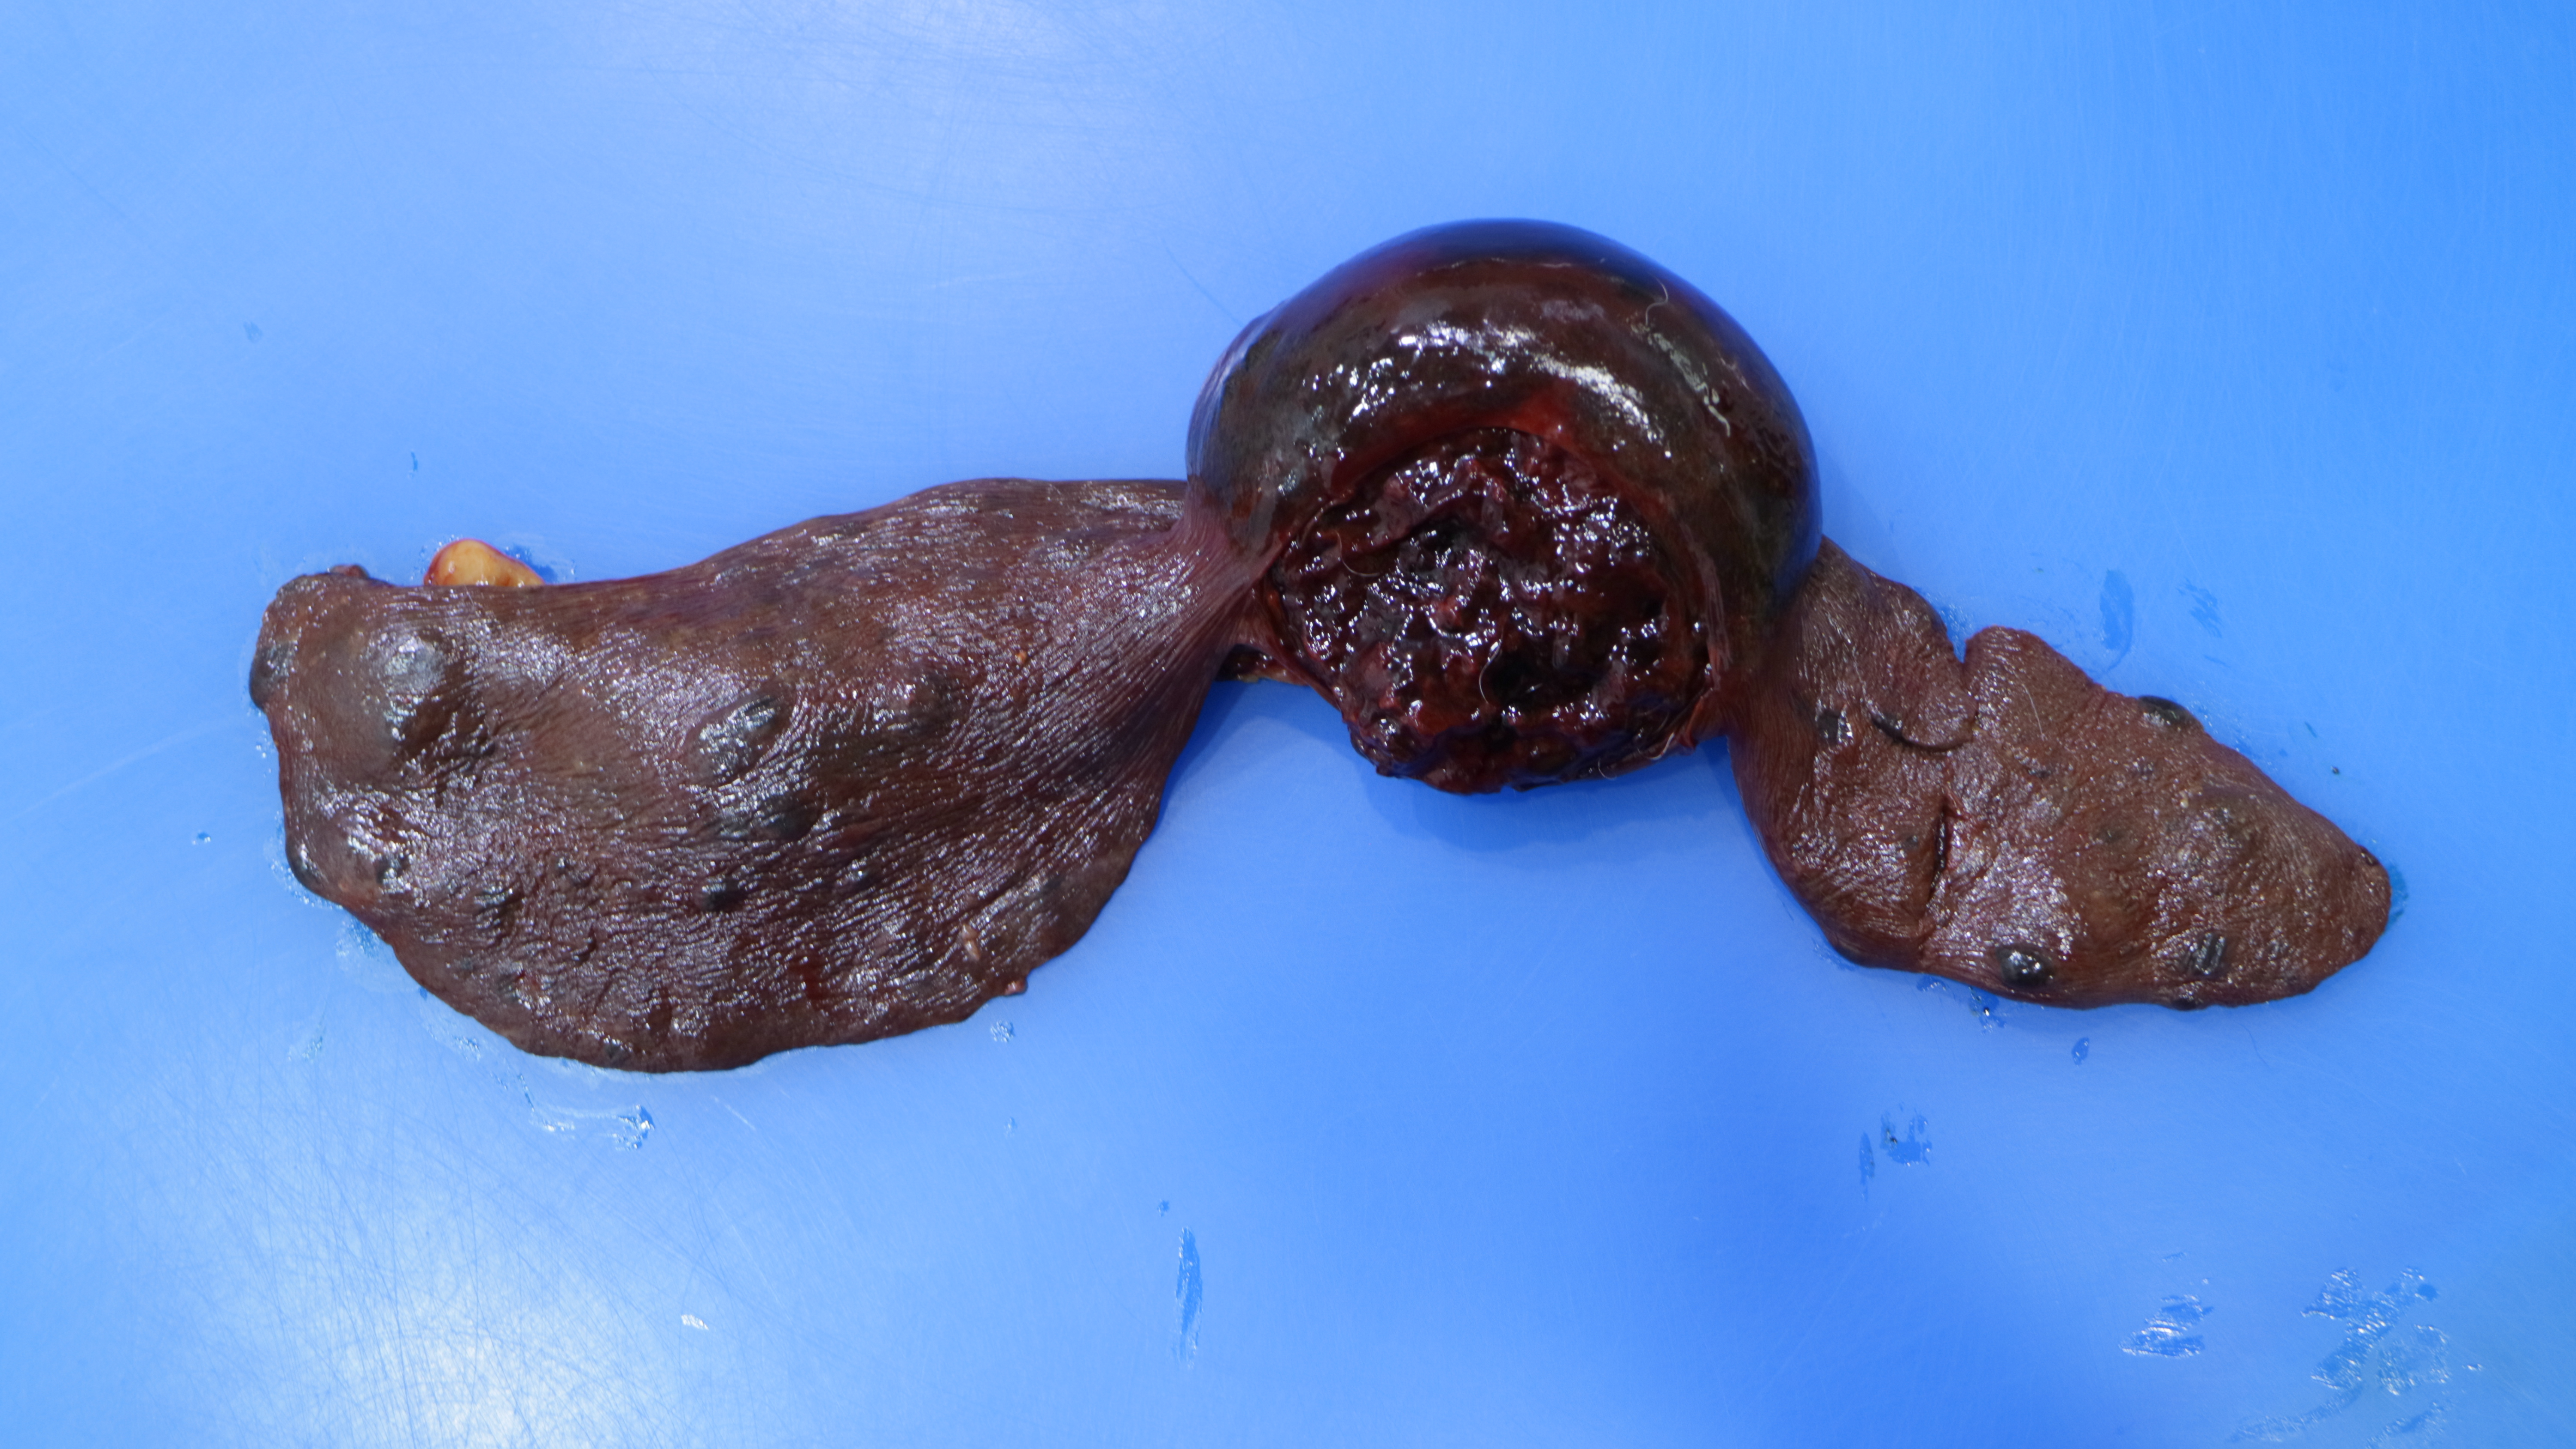
\includegraphics[width=1\linewidth]{images/spleen-hemangio-1} 

}

\caption{A large, red, friable, partially necrotic mass is present at the approximate midpoint of the spleen. Multiple other variably sized, red, raised masses are present randomly throughout the remaining parenchyma.}\label{fig:hemangio}
\end{figure}

Histologically, hemangiosarcomas are composed of thin-walled,
endothelial-lined channels filled with blood. As you can imagine, these
channels are fragile, and one of the most common and serious
complications of hemangiosarcoma is \textbf{rupture}, leading to
variably profound hemorrhage (hemoabdomen) and shock.

Hemangiosarcomas are very prone to metastasis, and frequently
metastasize to the \textbf{liver and lungs} (Fig
\ref{fig:hemangio-met}), as well as the heart and CNS. In the liver and
lungs, metastatic nodules are distinctive, small (\textasciitilde{} 1
cm), raised, spherical, red masses, colloquially referred to as
``cannonball'' lesions.

\begin{figure}

{\centering \includegraphics[width=1\linewidth]{images/liver-comp} 

}

\caption{A) A canine liver with multiple, variably sized, raised, roughly spherical masses protruding from the capsular surface. B) On cut section, the masses are red, geletinous, well-demarcated, and roughly spherical.}\label{fig:hemangio-met}
\end{figure}

\hypertarget{lymphoma}{\subsubsection{Lymphoma}\label{lymphoma}}

Lymphoma in the spleen is similar to that in other locations (see main
section on \protect\hyperlink{lymphoma}{Lymphoma}). There are uncommon
forms of primary splenic lymphoma that are generally slow growing and
tend to be limited to the spleen (e.g.~mantle zone and marginal zone
lymphomas), but these will not be covered here. Various leukemias can
also enlarge the spleen.

\subsubsection{Hemophagocytic histiocytic
sarcoma}\label{hemophagocytic-histiocytic-sarcoma}

This is a malignant neoplasm that often manifests with splenomegaly. It
is characterized by a diffusely meaty spleen, enlarged by huge numbers
of neoplastic macrophages. These macrophages phagocytose erythrocytes,
leading to anemia, often mimicing immune-mediated hemolytic anemia. It
is primarily a neoplasm of the dog, and may also affect the bone marrow.

\subsubsection{Non-angiomatous, non-lymphomatous
sarcomas}\label{non-angiomatous-non-lymphomatous-sarcomas}

This is a catch-all term for the large variety of other tumours that can
arise in the spleen. They are grouped together because they share a
similar gross and histological appearance, and, more importantly, a
similar clinical behaviour. They can be broadly divided into two
categories: clinically benign tumours, and their nefarious counterparts,
malignant and metastasizing masses. \textbf{Mitotic rate is the most
useful histologic feature in differentiating between the two}. The
survival time for animals with tumours of a high mitotic rate is
\emph{greatly decreased} as compared to those with low mitotic rates.
The liver is the most common site of metastasis.

\subsection{Miscellaneous conditions}\label{miscellaneous-conditions}

\subsubsection{Siderotic plaques}\label{siderotic-plaques}

\emph{Syn: Gamna-Gandy bodies, siderofibrotic plaques.}

These are \textbf{very common lesions} in the spleen of geriatric dogs,
and are thought to be the result of previous trauma or hemorrhage. They
are found in the splenic capsule, typically along the periphery but
often extending centrally, and are tan to brown to yellow, firm, and
dry. Their primary importance is in recognizing that \textbf{they are
incidental findings, of no clinical relevance}.

\subsubsection{Splenic rupture}\label{splenic-rupture}

Rupture of the spleen can be an acute, life threatening event, primarily
due to massive hemorrhage and hypovolemic shock. Prompt surgical
intervention is generally required. By far, the most common cause of
splenic rupture is trauma. Occasionally, splenic rupture is diagnosed in
the absence of trauma; in those cases, an underlying cause for abnormal
splenic fragility should be sought. In particular, neoplasms or other
growths may render the spleen more susceptible to rupture.

An interesting and occasional consequence of splenic rupture is the
so-called ``seeding'' of the abdomen with splenic tissue, which can
implant and develop functional capabilities. The presence of multiple
small splenic nodules throughout the abdomen is known as
\textbf{splenosis}. Be cautious, however, when you are faced with
interpreting this lesion: metastatic hemangiosarcoma can also present as
small red nodules throughout the mesentery, and they are very difficult
to distinguish grossly.

\hypertarget{biopsying-the-spleen}{\subsection{Biopsying the
spleen}\label{biopsying-the-spleen}}

Finally, a quick note on biopsies of the spleen. When a lesion is
discovered on the spleen, the usual clinical course is a complete
splenectomy. \textbf{The entire spleen is always the best sample to
send}, however, it is not always technically feasible. In cases where
the whole spleen cannot be sent, taking multiple samples of the
\textbf{junction of the mass (or lesion) and normal spleen} is the most
likely way to obtain a diagnosis. Many of these tumours, especially
hemangiosarcomas, have necrotic centers, and sampling the mass alone may
result in a dreaded ``non-diagnostic'' report. Note the word
``multiple'' above: the classical recommendation is that \emph{seven}
biopsies of a splenic mass are required to reliably rule out the
possibility of hemangiosarcoma (though a
\href{https://journals.sagepub.com/doi/full/10.1177/0300985819868732}{current
paper} suggests that perhaps 5 are adequate).

Splenic masses, in particular, often come in multiples. \textbf{They are
not guaranteed to be the same thing}. Therefore, \emph{each} mass should
be biopsied and submitted.

If a diffusely meaty spleen has been removed, send several 1 cm thick
samples.

\section{Lymph nodes}\label{lymph-nodes}

Lymph nodes are the waystations that lymph passes through on its way
back to the thoracic duct and general circulation. They are roughly
ovoid or renniform (``bean'' shaped), and are present in predictable
anatomic locations, some of which are superficial and \textbf{clinically
palpable}. They are critical tissues in the immune response of the
animal to pathogens, representing a major site for antigen presentation
and B-cell maturation.

As with all the other organs and systems in this section, a review of
the normal anatomy and function of the lymph node is useful. The
reference textbook (available electronically from the library) is
helpful.

Unlike other organs, where we typically go through diseases by process
(i.e.~inflammatory disease, neoplastic disease, etc), with lymph nodes
it is useful to separate diseases into those that make the lymph node
big (lymphadenopathies), and those that don't. As a rule of thumb,
\textbf{enlarged lymph nodes are much more significant than small lymph
nodes} to the point where ``lymphadenopathy'' generally refers to
enlarged lymph nodes (even though it strictly means ``disease of the
lymph node'').

\subsection{Lymphadenopathy}\label{lymphadenopathy}

There are \textbf{3 basic mechanisms that lead to enlargement of the
lymph node}. You should know them well.

\begin{enumerate}
\def\labelenumi{\arabic{enumi}.}
\tightlist
\item
  Infection of the lymph node itself
  (\protect\hyperlink{lymphadenitis}{lymphadenitis})
\item
  Reaction of the lymph node to infection
  (\protect\hyperlink{reactive-hyperplasia}{reactive hyperplasia})
\item
  Enlargement due to \protect\hyperlink{neoplasia-1}{neoplastic growth}
\end{enumerate}

The number and distribution of enlarged lymph nodes can be a helpful,
but not bulletproof, clue to the underlying etiology. For example,
enlargement of multiple lymph nodes from various anatomic locations
(e.g.~popliteal, superficial cervical, and submandibular) is suggestive
of neoplasia, whereas enlargement of a single lymph node may be more
indicative of lymphadenitis or reactive hyperplasia.

\hypertarget{lymphadenitis}{\subsubsection{Lymphadenitis}\label{lymphadenitis}}

Lymphadenitis refers to a lymph node that is \emph{infected}, which is
distinct from a lymph node that is reacting to infection elsewhere -
i.e., \protect\hyperlink{reactive-hyperplasia}{reactive hyperplasia}.
You should be able to confidently describe the differences between these
two conditions.

Lymphadenitis can be acute or chronic. It can be caseous, suppurative,
or granulomatous.

\paragraph{Acute lymphadenitis}\label{acute-lymphadenitis}

This may be the result of a regional lymph node draining an active
infection, and becoming infected in turn. If the infection is localized,
then a single lymph node may be affected. More generalized infections,
or septic animals, may have infection of multiple nodes. Affected lymph
nodes are enlarged, soft to firm, red, and often bulge on cut section.

\textbf{Strangles in horses is an important example of acute suppurative
lymphadenitis}. It is caused by \emph{Streptococcu equi} spp.
\emph{equi}. Following inhalation or direct contact with the organism,
there is colonization of the lymph nodes, particularly the
\textbf{mandibular and retropharyngeal} lymph nodes. Large abscesses
develop, and may rupture, draining pus and bacteria into the environment
or the guttural pouches. In a subset of cases, bacteria disseminate
through the lymph or blood to other organs (lung, liver, kidney,
mesenteric lymph nodes) and form similar lesions in a condition known as
\textbf{bastard strangles}.

\paragraph{Chronic lymphadenitis}\label{chronic-lymphadenitis}

These conditions are characterized by their longer duration and often
the presence of fibrosis. A few key diseases are discussed.

\textbf{Caseous lymphadenitis (CLA)} is primarily a disease of small
ruminants, though the causative agent, \emph{Corynebacterium
pseudotuberculosis}, also causes ulcerative lymphangitis in cattle and
horses. CLA in sheep almost always occurs following an injury from
shearing. Organisms then spread to local, draining lymph nodes, where it
develops into a chronic, suppurative to caseous infection. The disease
can then enter a cycle of abscess formation (characterized by a fibrous
capsule) followed by necrosis and reformation of an abscess. This
creates \textbf{characteristic concentric laminations}, considered to be
hallmarks of this disease. Once in the lymph node, this infection is
often persistent, and can spread slowly to internal organs. In goats,
CLA predominantly affects the lymph nodes of the head.

\textbf{Mycobacterium bovis}, the causative agent of bovine
tuberculosis, causes single to multiple discrete white areas of
\emph{granulomatous} inflammation in lymph nodes. The center of these
nodules often exhibits caseous necrosis. Lymph nodes are enlarged and
occassionally gritty on cut-section.

\textbf{Porcine circovirus 2} causes a variety of clinical syndromes,
including post-weaning multisystemic wasting syndrome. One manifestation
of viral disease is depletion of the lymphocytic population of the lymph
nodes, and enlargement with diffuse, granulomatous inflammation.

\hypertarget{reactive-hyperplasia}{\subsubsection{Reactive
hyperplasia}\label{reactive-hyperplasia}}

Reactive hyperplasia is the sterotypical, physiological reaction of a
lymph node to antigenic stimulation. It usually involves proliferation
of lymphocytes and expansion of the cortex or paracortex, but can
occasionally manifest as expansion of the sinuses with histiocytes. The
number of lymph nodes affected is variable and depends on the
location(s) of the initiating stimulus. Grossly, lymph nodes are
enlarged, pale, non-painful, and may bulge on cut-section.

Despite the brevity of this section, \textbf{this is a very common
finding in all domestic species}. Understanding that enlarged lymph
nodes are a \textbf{normal, immunological reaction to infections} is
important.

\hypertarget{neoplasia-1}{\subsubsection{Neoplasia}\label{neoplasia-1}}

\hypertarget{primary-neoplasia}{\paragraph{Primary
neoplasia}\label{primary-neoplasia}}

Lymphoma, lymphoma, lymphoma. \textbf{Lymphoma is one of the most common
malignant neoplasms of many domestic species}. Whether you practice
bovine, equine, or companion animal medicine, you will encounter
lymphoma. Chickens? Lymphoma. Wildlife? Usually infectious diseases, but
sometimes, lymphoma. It is worth taking your time to work through this
section (because you will need to know it, and because it will be on the
exam). As a sidenote, lymphoma is sometimes referred to as
lymphosarcoma. The two terms mean the same thing, and lymphoma is
currently the preferred term.

The classification of lymphomas is a complex, multifactorial process,
involving clinical, histopathological, immunohistochemical, and
molecular information. In reality, the diagnostic process often ends
with the diagnosis of `lymphoma', rather than pursuing the advanced
diagnostic modalities that would be commonplace in human medicine. The
current classification system was developed by the World Health
Organization, and includes around 35 different subtypes. Some practical
aspects of classification are useful to review.

\begin{enumerate}
\def\labelenumi{\arabic{enumi}.}
\tightlist
\item
  Anatomical location

  \begin{enumerate}
  \def\labelenumii{\roman{enumii})}
  \tightlist
  \item
    Multicentric: present in multiple lymph nodes, ± liver, spleen, bone
    marrow
  \item
    Cutaneous: in the skin
  \item
    Alimentary: within the gastrointestinal tract
  \item
    Hepatosplenic: in the liver and/or spleen
  \item
    Thymic: Affects the (you guessed it) thymus.
  \item
    Miscellaneous: ocular, hepatic, specific splenic forms, etc.
  \end{enumerate}
\item
  Immunophenotype: B or T cell, or neither (e.g NK cell).
\item
  Grade: based on histopathological features, usually mitotic count. A
  higher grade is associated with a \emph{poorer} prognosis.
\end{enumerate}

\textbf{Lymph nodes with lymphoma appear grossly enlarged and
homogenously pale white, occasionally streaked with hemorrhage. They are
typically firm. It is difficult to grossly distinguish between reactive
hyperplasia and lymphoma.}

There are key species differences when it comes to lymphoma.

\subparagraph{Canine}\label{canine}

\textbf{Lymphoma is the most common \emph{hematopoeitic} neoplasm of
dogs}. Large-breed dogs are predisposed, including Golden and Labdrador
retrievers and Boxers. Cocker spaniels, Terriers, and Beagles are also
overrepresented. Several forms of lymphoma occur in the dog, but
\textbf{multicentric is by far the most common}, usually presenting as a
\textbf{generalized lymphadenopathy, especially of the peripheral lymph
nodes}. They can be \textbf{either B- (more common) or T-cell in
origin}. Clinical signs are vague and are often absent during the early
stages of disease. Alimentary lymphoma occurs but is less common than in
cats. They are usually of \textbf{T-cell} origin, and often progress
slowly. Clinical signs relate to the GI tract: diarrhea, vomiting, and
weight loss. Cutaneous lymphomas, most commonly epitheliotropic T-cell
lymphoma, are about as common as GI lymphoma. They are often a cause of
pruritus, but gross lesions are varied and difficult to distinguish from
other causes of pruritus. Epitheliotropic lymphoma may affect the skin
or gums (Fig \ref{fig:epithelio}). The disease is slowly progressive. A
variety of other slowly progressive lymphomas affect the dog, but are
infrequent. Chemotherapy is available for many canine lymphomas with
varying degrees of success, but can often induce remission.

\begin{figure}

{\centering \includegraphics[width=1\linewidth]{images/epithelio} 

}

\caption{A) A poorly demarcated area of the gingival mucosa is deep red to purple, looking very much like an ecchymosis (bruise). B) Histology of this area reveals a neoplastic population of round cells infiltrating the epidermis and superficial dermis. The diagnosis was epitheliotropic lymphoma.}\label{fig:epithelio}
\end{figure}

\subparagraph{Feline}\label{feline}

\textbf{Lymphoma is the most common malignant neoplasm of cats, with
alimentary lymphoma being the most common anatomical type}. Other forms,
such as multicentric, nasopharyngeal, or mediastinal, occur, but with
far less frequency. Alimentary lymphoma in cats is usually of
\textbf{T-cell} origin (formally known as enteropathy-associated T-cell
lymphoma). This type of lymphoma typically progresses slowly, with
weight loss, diarrhea, and vomitting as the principle clincal signs. The
microscopic appearance of the disease is one of infiltrative lymphocytes
within the epithelium and lamina propria, and it can \textbf{therefore
be quite difficult to distinguish from inflammatory bowel disease}.
Submitting \textbf{full-thickness or deep-endoscopic biopsies} gives you
the best chance at a diagnosis. Many endoscopic biopsies are `wimpy' -
consisting of shallow portions of the superficial mucosa, giving the
pathologist little ability to distinguish between the two diseases. The
prognosis for this type of lymphoma is a bit controversial, as large
scale studies are still unavailable, but it is generally considered to
be a slowly `smoldering' disease that an animal may live with for a
significant amount of time.

Multicentric lymphoma is the next most common form in the cat, and
unlike in the dog, \textbf{involvement of the peripheral lymph nodes is
not a prominant feature}. Instead, liver and kidney are more commonly
involved.

Historically, feline lymphoma was \textbf{highly associated with the
prevalance of feline leukemia virus}, and testing and control of FeLV
has greatly reduced the incidence of lymphoma, particularly thymic and
multicentric lymphomas, in younger cats. FIV has also been associated
with lymphoma.

\subparagraph{Bovine}\label{bovine}

Lymphoma in cows is separated into two major forms:

\begin{enumerate}
\def\labelenumi{\arabic{enumi}.}
\tightlist
\item
  \textbf{Enzootic bovine leukosis:} Caused by bovine leukemia virus
  (BLV), a retrovirus that infects \textbf{B-cells}. The virus is
  transmitted horizontally, mostly by infected arthropods,
  iatrgoenically (re-use of needles, rectal sleeves), colostrum/milk
  administration, or natural breeding. The virus causes
  \textbf{multicentric lymphoma in cattle 5-8 years old}. Like all
  retroviruses, once the virus has infected the host, infection is
  lifelong, but \emph{infection does not necessarily result in
  lymphoma}. Of the infected animals, around 30 \% will develop a
  persistant lymphocytosis, and of those, around 5 \% will develop
  lymphoma. Animals that present with the disease typically have
  markedly enlarged lymph nodes, nodules in the heart (Fig
  \ref{fig:leukosis-heart}), abomasum, uterus, and the vertebral canal.
  Clinical signs depend on the extend to which the neoplasm affects the
  various organs.
\item
  \textbf{Sporadic lymphoma}: these are associated with younger cattle
  \textbf{and are not associated with BLV}. They are usually of
  \textbf{T-cell origin}.

  \begin{enumerate}
  \def\labelenumii{\roman{enumii})}
  \tightlist
  \item
    Juvenile, multicentric: Typically found in calves 3 - 6 months old.
    Virtually all lymph nodes are affected, and as well as bone marrow,
    leading to myelopthisis and pancytopenia. Visceral organs may be
    invovled.
  \item
    Thymic: Typically in cattle \textless{} 2 years old, thymic lymphoma
    may cause pre-sternal swelling leading, jugular distension, and
    local edema. As the tumour grows, compression of the lungs may lead
    to respiratory difficulty.
  \item
    Cutaneous: Typically in cattle 2 - 3 years old, this is the
    \textbf{least common form of lymphoma}. Presents with round, raised,
    plaques along the head, sides, and perineum that often ulcerate. The
    disease may wax and wane, but eventually progresses to involve
    visceral organs (indistinguishable from enzootic bovine leukosis).
  \end{enumerate}
\end{enumerate}

\begin{figure}

{\centering \includegraphics[width=1\linewidth]{images/bovine-leukosis-heart} 

}

\caption{In this example of bovine leukosis, there are multiple raised white nodules throughout the myocardium of this heart (you are looking into the opened left atrium and ventricle). Photo courtesy of J. Schenkels.}\label{fig:leukosis-heart}
\end{figure}

\subparagraph{Equine}\label{equine}

\textbf{Lymphoma is the most common malignant neoplasm of the horse}.
Most are \textbf{B-cell} in origin and are multicentric. Note that in
the horse, the multicentric form typically forms masses in the abdomen
and thorax, as well as the subcutis, but \textbf{not typically a
generalized lymph adenopathy}. Alimentary and cutaneous forms also
occur, and both are usually T-cell in origin. Horses with any form of
lymphoma will typically present with clinical signs of ill-thrift,
anorexia, depression, and pyrexia. Colic may occur with alimentary or
multicentric lymphoma. Quarter horses and Thoroughbreds most often
develop multicentric lymphoma, while Standardbreds have a higher
incidence of alimentary lymphoma.

\subparagraph{Porcine}\label{porcine}

\textbf{Lymphoma is the most common neoplasm in pigs}, but data is
lacking regarding the most common type. Multicentric (affecting
visceral, rather than peripheral, lymph nodes) and thymic are most
common. Affected animals are often young (\textless{} 1 year).

\subparagraph{Avian}\label{avian}

Poultry are affected by two different forms of lymphoma. Both are caused
by virally-induced malignant transformation of lymphocytes.

\begin{enumerate}
\def\labelenumi{\arabic{enumi}.}
\tightlist
\item
  \textbf{Marek's disease} primarily occurs in younger birds (four weeks
  and older), and is of \textbf{T-cell origin}. It is caused by Gallid
  herpesvirus 2, for which a vaccine is available. It causes lymphoma in
  a wide variety of organs, but particularly prominently in the nerves
  (e.g.~sciatic nerves), leading to the classic clinical sign of uni- or
  bilateral hind-limb paralysis. The eyes, visceral organs, and skin are
  often also affected, but the \emph{bursa of Fabricius is usually
  spared}.
\item
  \textbf{Avian leukosis} is caused by a retrovirus and transforms
  \textbf{B-cells}. Due to the nature of the virus, disease does not
  usually manifest until the animal is older than 14 weeks. The virus
  causes lymphoma in a variety of organs, including the bursa of
  Fabricius, liver, spleen, and kidney. Distinguishing between avian
  leukosis and Marek's disease in an older chicken is challenging with
  histopathology alone and generally requires ancillary diagnostics.
\end{enumerate}

\paragraph{Metastatic}\label{metastatic}

The lymph nodes are a very common site for metastases from a wide
variety of neoplasms (carcinomas, mast cell tumours, oral malignant
melanomas, for example). The gross appearance of the lymph node will
vary somewhat depending on the primary neoplasm, but in general they are
enlarged, firm, and may be mottled on cut section. Metasases will appear
first in the closest draining lymph nodes.

\subsection{Lymph node atrophy}\label{lymph-node-atrophy}

As noted above, small lymph nodes are uncommonly a sign of pathology.
Primary causes of small lymph nodes include:

\begin{enumerate}
\def\labelenumi{\arabic{enumi}.}
\tightlist
\item
  Atrophy associated with aging (senile atrophy)
\item
  Cachectic atrophy, seen in animals
\end{enumerate}

\section{Thymus}\label{thymus}

The thymus is responsible for the training of T-cells, ensuring that
self-reactive T-cells are removed from circulation. The thymus is at its
largest and most active in neonatal and young animals, where it forms a
large, multilobular, intrathoracic organ in the cranial mediastinum. As
you'll recall, the thymus regresses over the lifetime of an animal,
becoming practically inapprent by the time most animals have reached
sexual maturity. Although still present, at this stage the thymus is
typically indistinguishable from the mediastinal fat.

It is broken down into lobules composed of a cortex and medulla, and has
both an epithelial and lymphoid component.

With the exception of a few diseases, thymuses tend not to be a primary
source of clincial disease.

\subsection{Miscelaneous conditions}\label{miscelaneous-conditions}

\subsubsection{Atrophy}\label{atrophy}

Thymic atrophy is one of the most common chagnes noted in the thymus.
Two basic pathogenic mechanisms can lead to thymic atrophy. Because the
lymphoid population of the thymus is compsoed of precursor cells from
the bone marrow, destruction of precursor cells in the bone marrow can
lead to atrophy of the thymus. The second mechanism is direct damage to
the lymphocytes within the thymus itself. Causes include viral infection
(e.g.~BVDV, canine distemper virus, FIV, canine and feline parvovirus,
EHV-1, and classical swine fever virus), toxins, chemotherapy, and
radiation. Care must be taken when deciding if the thymus is atrophied:
the thymus naturally involutes with age, and thus age-matched controls
are often necessary to grossly identify atrophy.

\subsubsection{Hypoplasia}\label{hypoplasia-1}

Recall that aplasia signifies failure of an organ to reach its normal
size (contrast this with atrophy, in which organ has at one point been
normal, but has then become smaller). Aplasia of the thymus is a
congenital defect, usually involving an immunodeficiency of T cells. The
most common manifestation of thymic hypoplasia is part of \emph{severe
combined immunodeficiency} syndrome in foals, particularly Arabians, and
certain breeds of dogs (Jack Russell terriers, Bassett hounds). The
thymus of these animals is devoid of lymphocytes, rendering them
markedly small. These animals are predisposed to infection and
frequently do not live long after birth.

\subsubsection{Hemorrhage}\label{hemorrhage}

Massive thymic hemorrhage is an uncommon but important finding
particularly in dogs, where it can be the only lesion. Three main causes
are implicated, and should be included in a differential list:

\begin{itemize}
\tightlist
\item
  Anticoagulant rodenticides
\item
  Trauma
\item
  Idiopathic
\end{itemize}

These three causes are indistinguishable on gross examination, and would
require additional history and/or toxin testing. The degree of
hemorrhage can be profound and life threatening.

\subsection{Thymic neoplasia}\label{thymic-neoplasia}

The thymus has an \textbf{epithelial and a lymphoid component}, and
either may give rise to a neoplasm. Neoplastic proliferations of
lymphocytes are of course lymphomas, while in the thymus, epithelial
neoplasms are known as thymomas.

\subsubsection{Thymic lymphoma}\label{thymic-lymphoma}

Unsurprisingly, thymic lymphoma is almost always T-cell in origin. It
usually affects younger animals, particularly \textbf{cats, calves}, and
less commonly dogs. \textbf{In young cats, thymic lymphoma is highly
associated with feline leukemia virus (FeLV)}, and the widespread
vaccination of cats against this virus has dramatically decreased the
incidence of the disease in these animals. There is no viral association
in other animals, or in older cats.

Grossly, the neoplasm is generally present diffusely throughout the
thymus, creating a large, space-occupying mass in the mediastinum. The
mass may get large enough that it compresses the lungs, resulting in
dyspnea. Thoracic effusion is also frequently present.

\subsubsection{Thymoma}\label{thymoma}

This neoplasm of the epithelial component of the thymus is most
frequently seen in dogs and small ruminants (sheep, goats). They tend to
be slow-growing, relatively benign tumorus that only rarely metastasize.
They are grossly indistinguishable from thymic lymphoma, thus,
\textbf{histopathology is required to differentiate between the two}.
Dogs with thymomas often develop
\href{http://russfraser.ca/muscle/immune-mediate-myopathies.html\#acquired-myasthenia-gravis}{myasthenia
gravis} (note: link takes you to a separate package of course notes on
skeletal muscle. The details of myasthenia gravis are \emph{not}
required for exams on the hemolymphatic system).

\bibliography{book.bib,packages.bib}


\end{document}
